\documentclass[11pt,letterpaper]{article}
\usepackage[english]{babel}
\usepackage[utf8]{inputenc}
\usepackage{fancyhdr}
\usepackage[margin=1in]{geometry}
\usepackage{enumitem}
\usepackage{amsmath}
\usepackage{graphicx}
\usepackage{setspace} 
\usepackage{pdfpages}
\usepackage{xcolor}
\onehalfspacing
 
\pagestyle{fancy}
\fancyhf{}
\lhead{AMATH 383 HW 3}
\rhead{Nan Tang (1662478)}
\rfoot{Page \thepage}
 

\title{AMATH 383 HW 3}
\author{Nan Tang 1662478}
\date{\today}
 
 
\begin{document}
\maketitle

\section*{Exercise 6.6}
\subsection*{a}
\noindent Let $\frac{dp}{dt} = f(p) = 0$, then we get the equation
\begin{align*}
f(p) = \alpha p(1 - p) (p - \frac{1}{2}) = 0
\end{align*}
\noindent Since $\alpha \neq 0$, equilibrium points are $p = 0, p =\frac{1}{2}, p = 1$.
\begin{align*}
\frac{d f(p)}{dp} &= \alpha (- (x - \frac{1}{2}) x + (1 - x)x + (1 - x)(x - \frac{1}{2})) \\
&= \alpha (- \frac{6x^2 - 6x + 1}{2})
\end{align*}
\noindent At $p = 0, f(p)' = - \frac{1}{2} \alpha$, at $p = \frac{1}{2}, f(p)' = \frac{1}{2} \alpha$, at $p = 1, f(p)' = - \frac{1}{2} \alpha$
\noindent Since in the past and in the present, right handed snail are always commoner than left handed, $p = 1$ where probability of right handed snail is approximately $100 \%$ should be a stable point. This indicates $f(p)'$ at $p = 1$ should have negative sign, i.e. $\alpha > 0$. \\

\noindent Thereby we get $p = 0, f(p)' < 0$, at $p = \frac{1}{2}, f(p)' > 0$, at $p = 1, f(p)' < 0$. $p = 0, 1$ are stable points, while $p= \frac{1}{2}$ is unstable point. 


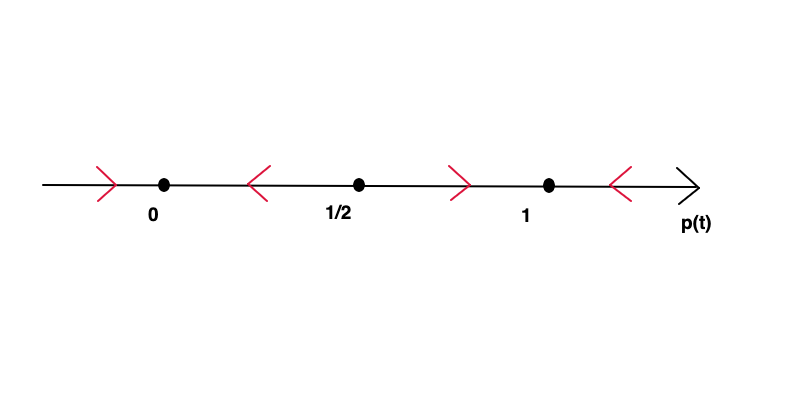
\includegraphics[scale=0.3]{hw3-1.png}

\subsection*{b}
\noindent Note that $p = \frac{1}{2}$ is an unstable point. For any initial value of $p$ that greater than $\frac{1}{2}$, as $t \rightarrow \infty$, $p(t)$ will asymptotically go to 1 (all right handed); for any initial value of $p$ less than $\frac{1}{2}$, $p(t)$ will asymptotically go to 0 (all left handed). Therefore with initial condition $p(0) = \frac{1}{2}$, there is $50 \%$ chance all snails are left handed in hundred million years, and $50 \%$ chance all snails are right handed. 

\section*{Exercise 6.8}
\noindent Base on given information, the epidemic model should be 
\begin{align*}
\frac{d I}{dt} &= \alpha I(t) N(t) \\
&= \alpha I(t) (1000 - I(t))
\end{align*}
\noindent At $I = 100, \frac{dI}{dt} = 90$,
\begin{align*}
90 &= \alpha \cdot 100 (1000 - 100) \\
\alpha &= \frac{1}{1000} \\
\frac{dI }{dt} &= \frac{1}{1000} I(t) (1000 - I(t))
\end{align*}
\noindent This is a separable ODE, solve by separate integral, and partial fraction
\begin{align*}
\int \frac{1}{I (1000 - I)} dI &= \int \frac{1}{1000} dt \\
\int \frac{1}{1000} (\frac{1}{I} + \frac{1}{1000 - I}) dI &= \int \frac{1}{1000} dt \\
\int \frac{1}{I} + \frac{1}{1000 - I} dI &= \int 1 dt \\
ln|I| - ln|1000 - I| & = t + c \\
\frac{I}{1000 - I} &= e^{t + c} \\
I &= \frac{1000}{1 + e^{-t-c}}
\end{align*}
\noindent Plug in initial condition $I(0) = 20$ 
\begin{align*}
20 &= \frac{1000}{1 + e^{-c}} \rightarrow e^{-c} = 49 \\
I(t) &= \frac{1000}{1 + 49 e^{-t}}
\end{align*}
\noindent When $I = 900$ 
\begin{align*}
900 &= \frac{1000}{1 + 49 e^{-t}} \\
t &= ln(49) + ln(9) \approx 6.09
\end{align*}
\noindent After $6.09$ days, $90 \%$ population will be infected.

\section*{Exercise 9.6}
\noindent Plug in $P = pH - cE$ and $H = qEN$ into equations of $\frac{dE}{dt}, \frac{dN}{dt}$
\begin{align*}
g(E, N) &= \frac{dE}{dt} = apgEn - acE \\
f(E, N) &= \frac{dN}{dt} = rN(1 - \frac{N}{K}) - q EN
\end{align*}
\noindent Equilibrium points are when both $g(E, N)$ and $f(E, N)$ are zero. \\

\noindent There are overall three equilibrium points $(E^*, N^*) = (0, 0)$, $(E^*, N^*) = (0, K)$, $(E^*, N^*) = (\frac{r}{q} (1 - \frac{c}{Kpq}), \frac{c}{pq})$

\begin{align*}
a_{11} &= \frac{\partial f}{\partial N} = r - \frac{2rN}{K} - qE \\
a_{12} &= \frac{\partial f}{\partial E} = - qN \\
a_{21} &= \frac{\partial g}{\partial N} = a p q E \\
a_{22} &= \frac{\partial g}{\partial E} = apqN - ac
\end{align*}

\noindent Case 1: $(E^*, N^*) = (0, 0)$ \\

$a_{11} = r $, $a_{12} = 0$, $a_{21} = 0$, $a_{22} = -ac$ \\

$p = a_{11} + a_{22} = r - ac$, $q = a_{11}a_{22} - a_{12} a_{21} = -acr$ \\

$\lambda_1 = \frac{p}{2} + \frac{\sqrt{p^2 - 4q}}{2}  = r$ \\

$\lambda_2 = \frac{p	}{2} - \frac{\sqrt{p^2 - 4q}}{2} = -ac$ \\

\noindent since $r > 0$ therefore $\lambda_1 > 0$, it is an unstable point. \\

\noindent Case 2: $(E^*, N^*) = (0, K)$ \\

$a_{11} = -r $, $a_{12} = -qK$, $a_{21} = 0$, $a_{22} = apqK - ac$ \\

$p = a_{11} + a_{22} = -r + apqK - ac$, $q = a_{11}a_{22} - a_{12} a_{21} = -rapqK + rac$ \\

$\lambda_1 = \frac{p}{2} + \frac{\sqrt{p^2 - 4q}}{2}  = \frac{-r + apqK - ac}{2} + \frac{r + apqk - ac}{2} = apqK - ac$  \\

Note that $\frac{c}{pqK} < 1 \rightarrow c < pqK$, therefore $\lambda_1 > 0$

$\lambda_2 = \frac{p	}{2} - \frac{\sqrt{p^2 - 4q}}{2} = -r < 0$ \\

\noindent Since $\lambda_1 > 0$, it is an unstable point. \\

\noindent Case 3: $(E^*, N^*) = (\frac{r}{q} (1 - \frac{c}{Kpq}), \frac{c}{pq})$ \\

$a_{11} = - \frac{rc}{Kpq} $, $a_{12} = - \frac{c}{p}$, $a_{21} = apr - \frac{acr}{Kq}$, $a_{22} = 0$ \\

$p = a_{11} + a_{22} = - \frac{rc}{Kpq}$, $q = a_{11}a_{22} - a_{12} a_{21} = acr  - \frac{arc^2}{Kpq}$ \\

Note that $q = acr(1 - \frac{c}{Kpq}) > 0$ since $\frac{c}{Kpq} < 1$. Then $p^2 - 4q < p^2 \rightarrow |\frac{p}{2}| > |\frac{\sqrt{p^2 - 4q}}{2}|$. \\

$\lambda_1 = \frac{p}{2} + \frac{\sqrt{p^2 - 4q}}{2} < 0$ since $p < 0$ and $|\frac{p}{2}| > |\frac{\sqrt{p^2 - 4q}}{2}|$ \\

$\lambda_2 = \frac{p}{2} - \frac{\sqrt{p^2 - 4q}}{2} < 0$ since $p < 0,  - \frac{\sqrt{p^2 - 4q}}{2} < 0$ \\

Both $\lambda_1$ and $\lambda_2 < 0$, this point $(E^*, N^*) = (\frac{r}{q} (1 - \frac{c}{Kpq}), \frac{c}{pq})$ is a stable point. 



\end{document}